\chapter[Metodologia]{metodologia}

O Business Model Canvas, mais conhecido como Canvas, é uma ferramenta de planejamento estratégico, que permite desenvolver e esboçar modelos de negócio novos ou existentes. O uso desse modelo é indicado pelo SEBRAE.

Na primeira reunião de grupo  preenchemos o Canvas Fig. \ref{Canvas} de forma democrática e colaborativa, com toda a equipe. Dessa forma nos conhecemos melhor e motivamos todos a se envolver com as etapas do projeto. Além de conhecer nossos desafios e poder enfrentá-los sabendo os requisitos de cada área. 


 \begin{figure} [!htp]
	\centering
	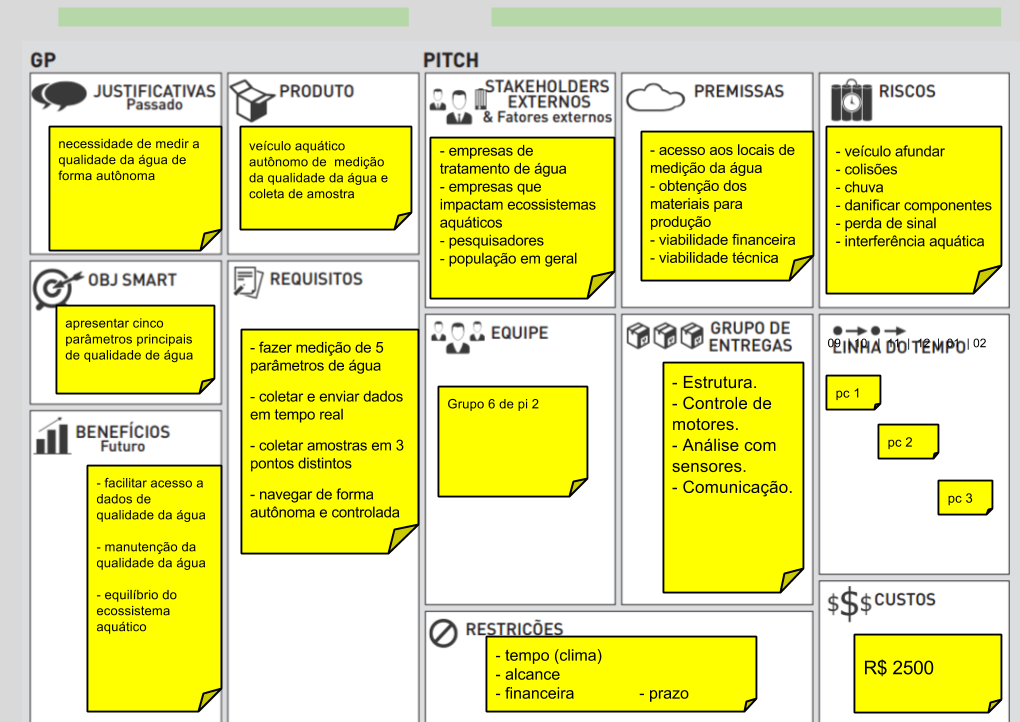
\includegraphics[scale=0.3]{figuras/Canvas}
	\caption{Ferramenta de planejamento estratégico chamada de Canvas. Business Model Canvas composto de 13 quadros.}
	\label{Canvas}
\end{figure}